\section{definition7}
\begin{definition}
\end{definition}

Suppose we have the following diagram of alternating $m$ red strands($R_1 - R_m$) and $m$ blue strands($B_1 - B_m$) labeled from the top:

\begin{figure}[H] % Optional: [h] means here, [t] for top, [b] for bottom, [p] for page of floats
    \centering
    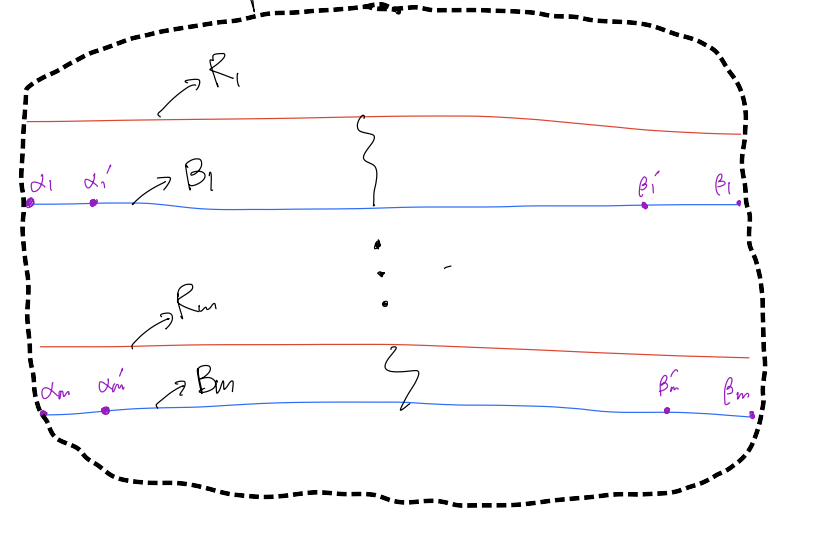
\includegraphics[width=\linewidth]{diagrams/definition7/1.png} % Adjust the width as needed
    \caption{Your caption here}
    \label{fig:your-label}
\end{figure}

We define MOVE \RN{7}-(a) inductively so that the final diagram looks as follows:

\begin{figure}[H] % Optional: [h] means here, [t] for top, [b] for bottom, [p] for page of floats
    \centering
    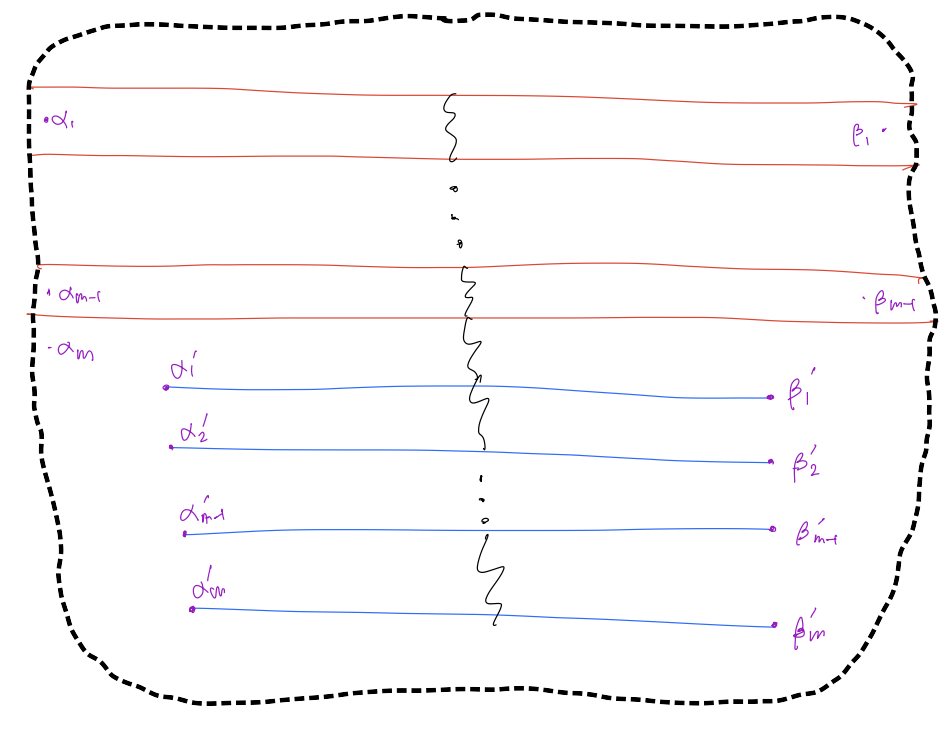
\includegraphics[width=\linewidth]{diagrams/definition7/2.png} % Adjust the width as needed
    \caption{Your caption here}
    \label{fig:your-label}
\end{figure}

We define MOVE \RN{7}-(a) inductively on $m$.
If $m=1$, then MOVE\RN{7}-(a) is the null move. If $m>1$,
(Step1) Apply MOVE\RN{7}-(a) to the first $m-1$ blue and red strands($B_1 - B_{m-1}$ and $R_1 - R_{m-1}$)(this has been defined by the induction hypothesis), we get :

\begin{figure}[H] % Optional: [h] means here, [t] for top, [b] for bottom, [p] for page of floats
    \centering
    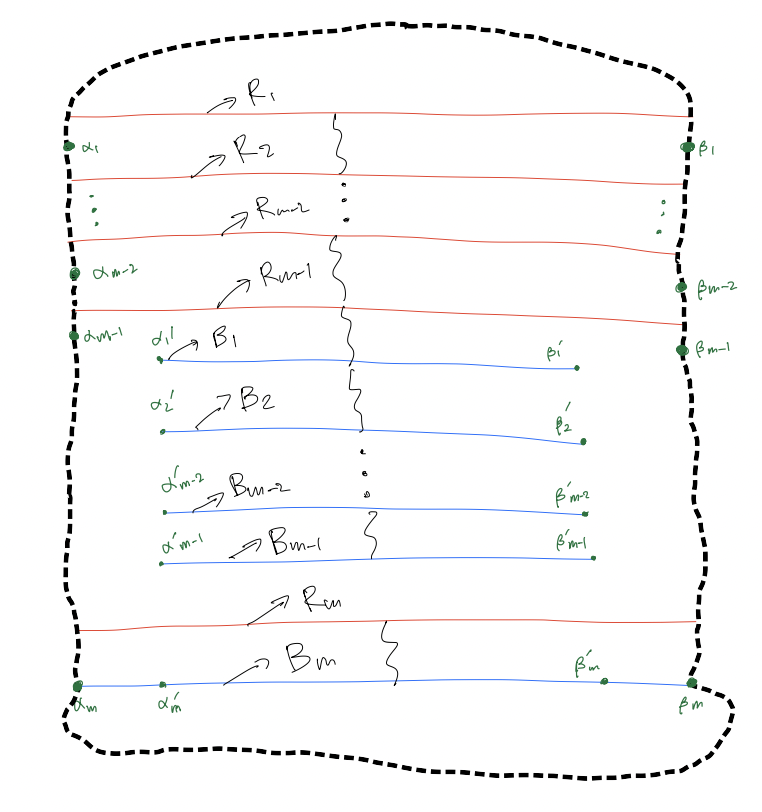
\includegraphics[width=\linewidth]{diagrams/definition7/3.png} % Adjust the width as needed
    \caption{Your caption here}
    \label{fig:your-label}
\end{figure}

(Step2) Apply MOVE \RN{6} to $B_1 - B_{m-1}$ and $R_m$, we get :
\begin{figure}[H] % Optional: [h] means here, [t] for top, [b] for bottom, [p] for page of floats
    \centering
    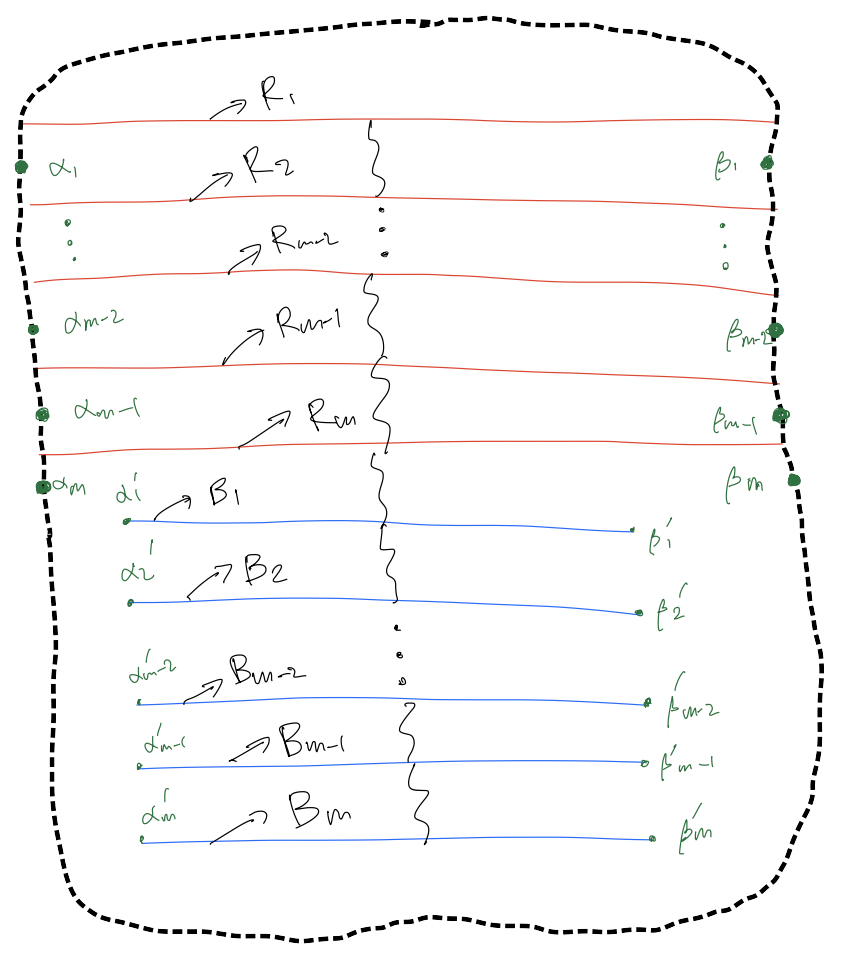
\includegraphics[width=\linewidth]{diagrams/definition7/4.png} % Adjust the width as needed
    \caption{Your caption here}
    \label{fig:your-label}
\end{figure}
By induction, we have defined MOVE \RN{7}-(a) for all $m\in \mathbb{M}$.

(b) Suppose we have the following diagram of $n$ red strands($R_1 - R_n$) and $m$ blue strands($B_1 - B_m$) labeled from the top :
\begin{figure}[H] % Optional: [h] means here, [t] for top, [b] for bottom, [p] for page of floats
    \centering
    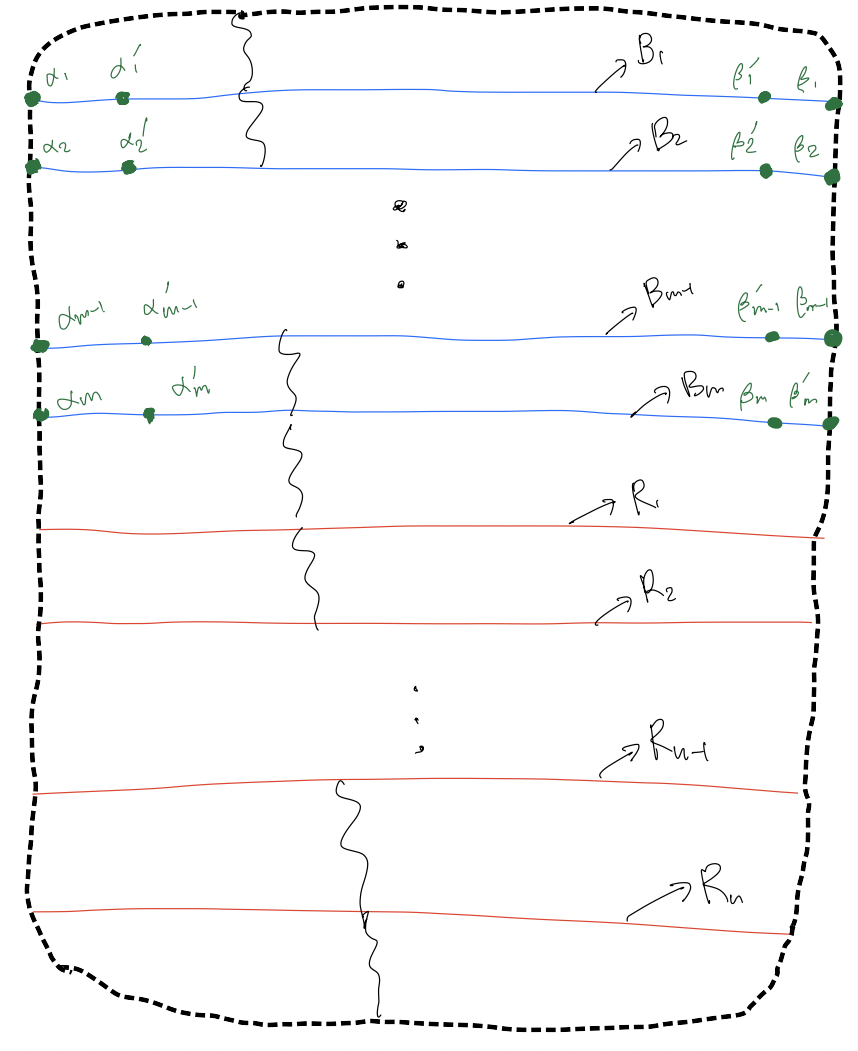
\includegraphics[width=\linewidth]{diagrams/definition7/5.png} % Adjust the width as needed
    \caption{Your caption here}
    \label{fig:your-label}
\end{figure}

We define MOVE \RN{7}-(b) inductively so that the final diagram looks as follows:
\begin{figure}[H] % Optional: [h] means here, [t] for top, [b] for bottom, [p] for page of floats
    \centering
    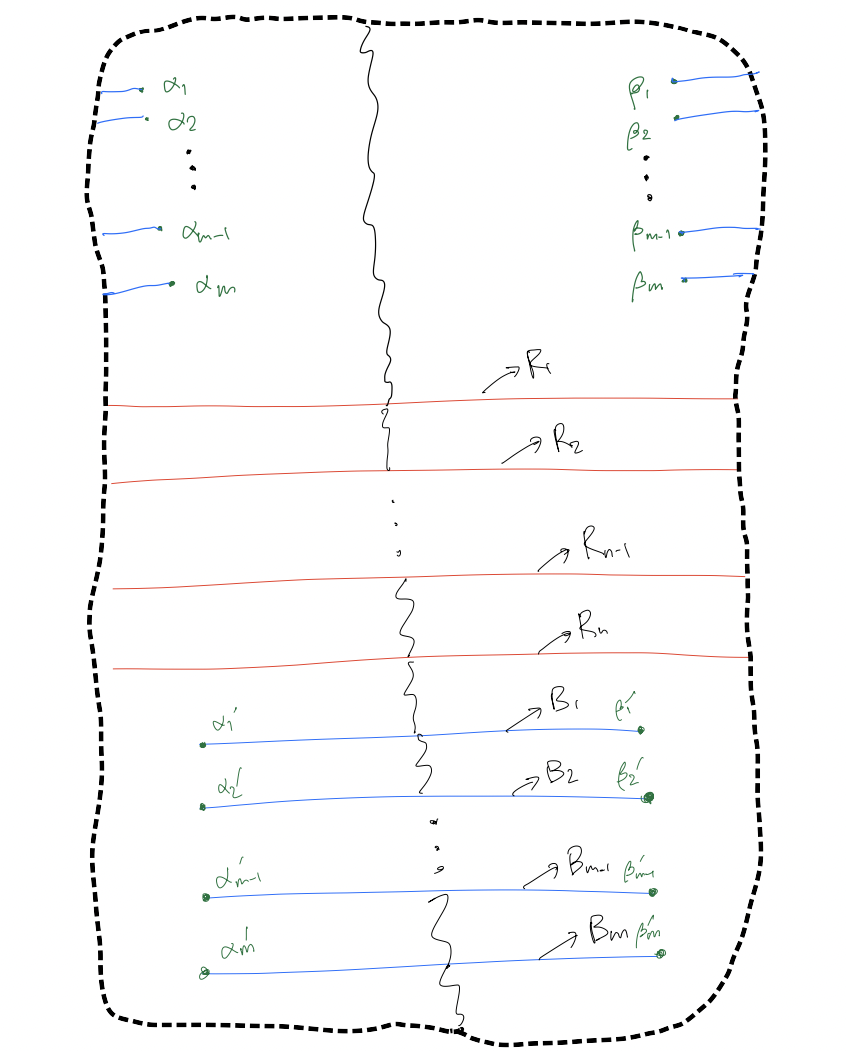
\includegraphics[width=\linewidth]{diagrams/definition7/6.png} % Adjust the width as needed
    \caption{Your caption here}
    \label{fig:your-label}
\end{figure}

We define MOVE \RN{7}-(b) inductively on $n$. If $n=1$, then MOVE \RN{7}-(b) is MOVE \RN{6}. If $n>1$, 
(Step1) apply MOVE \RN{7}-(b) to the first $m$ blue strands($B_1 - B_m$) and $n-1$ red strands($R_1 - R_{n-1}$)(this has been defined by the induction hypothesis), we get :
\begin{figure}[H] % Optional: [h] means here, [t] for top, [b] for bottom, [p] for page of floats
    \centering
    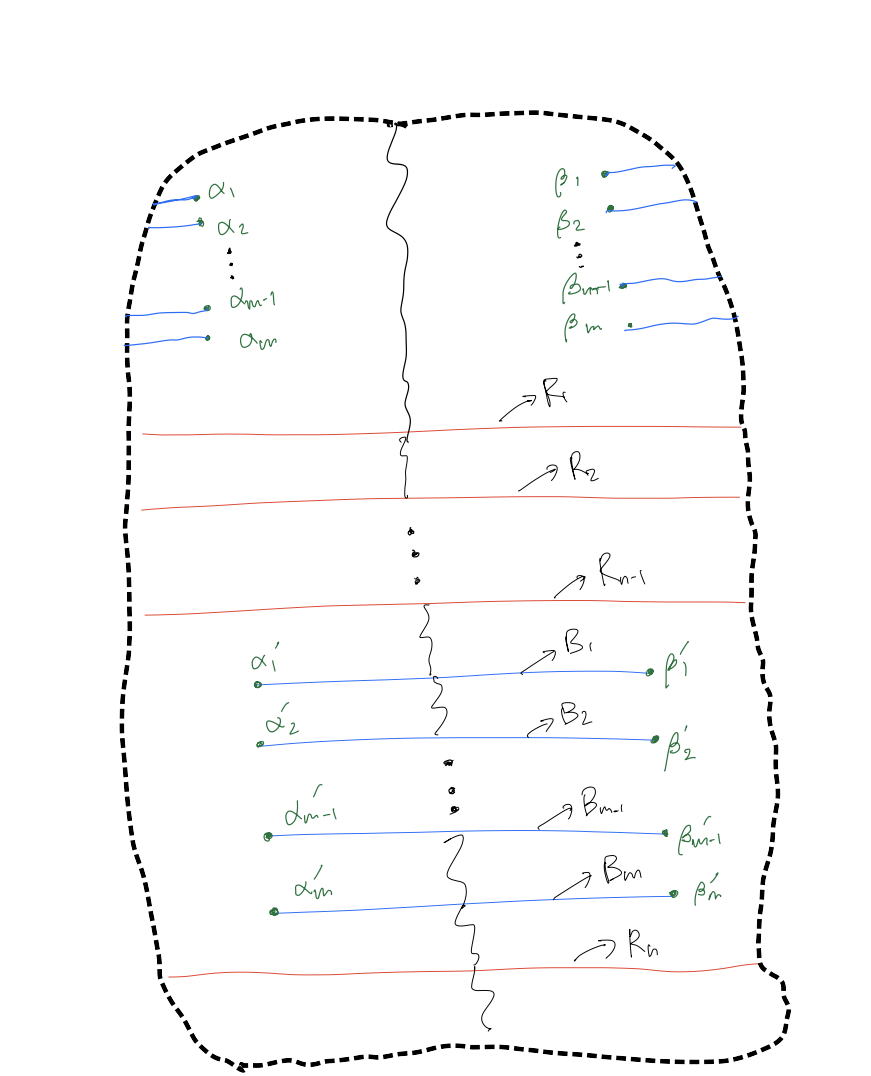
\includegraphics[width=\linewidth]{diagrams/definition7/7.png} % Adjust the width as needed
    \caption{Your caption here}
    \label{fig:your-label}
\end{figure}

(step2) apply MOVE \RN{6} to be $B_1 - B_m$ and $R_n$, we get the final diagram :
\begin{figure}[H] % Optional: [h] means here, [t] for top, [b] for bottom, [p] for page of floats
    \centering
    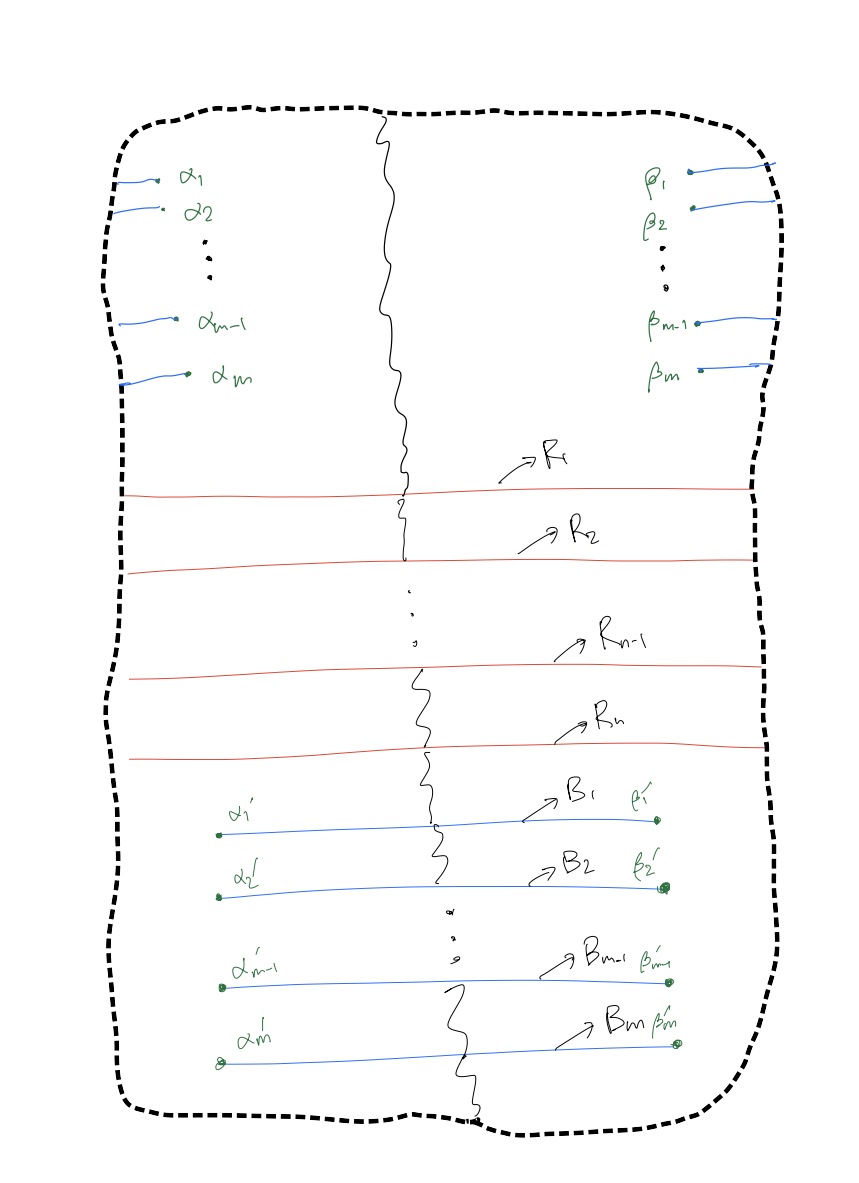
\includegraphics[width=\linewidth]{diagrams/definition7/8.png} % Adjust the width as needed
    \caption{Your caption here}
    \label{fig:your-label}
\end{figure}

By induction, we have defined MOVE \RN{7}-(b) for all $m\in \mathbb{N}$.